\documentclass{article}

\usepackage[main=english,vietnamese]{babel}
\usepackage[T1]{fontenc}
\usepackage[utf8]{inputenc}
\usepackage[sexy]{evan}
\usepackage{matchsticks}
\usepackage{wrapfig}
\usepackage{listings}

\newtheorem{hint}{Hint}

\title{A picture is worth a thousand words - Part 4}
\author{Nghia Doan}
\date{\today}

\begin{document}

\maketitle

This article is the fourth part of the series on investigating a number of ways to \textit{prove area equality without writing lengthy proof.}

\begin{example*}[Example 16]
    $ABCD$ and $DEFG$ are two squares as shown below, prove that
    \[
        [ADG] = [CDE].
    \]
\end{example*}

\begin{figure}[h]
    \centering
    \begin{minipage}[t]{6.5cm}
        \begin{center}
            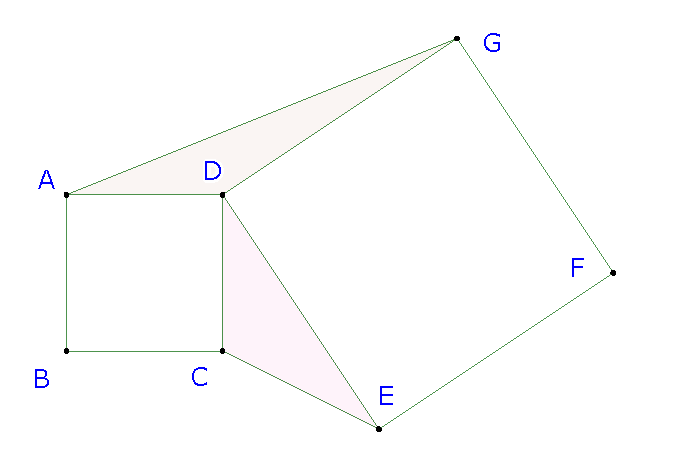
\includegraphics[width=6.5cm]{./svg/pdf/23-24-s3-i-p17.pdf}
        \end{center}
    \end{minipage}
    \qquad
    \begin{minipage}[t]{6.5cm}
        \centering
        \begin{center}
            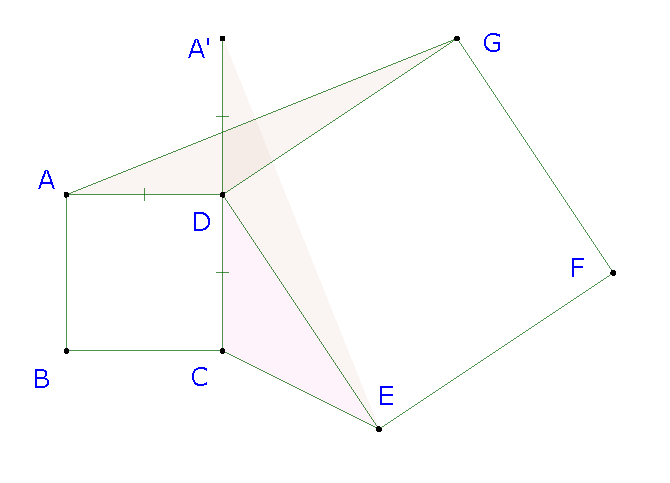
\includegraphics[width=6.5cm]{./svg/pdf/23-24-s3-i-p17-s.pdf}
        \end{center}
    \end{minipage}
\end{figure}

\begin{proof}
    Rotate the triangle $ADG$ clockwise around $D.$ Because $\angle CDA = \angle EDG = 90\dg,$ $DG = DE,$ we receive the triangle $A'DE.$
    $A', D, C$ are collinear (lie on the same line). Thus $[ADG] = [A'DE] = [DCE].$
\end{proof}

\newpage

\begin{example*}[Example 17]
    A half cirle and two quarters of circles are draw in a square as shown below.
    Find the ratio of the area of the shaded region to the area of the square.
\end{example*}

\begin{figure}[h]
    \centering
    \begin{minipage}[t]{6.5cm}
        \begin{center}
            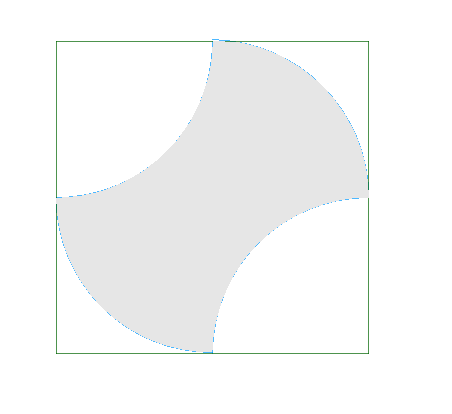
\includegraphics[width=5.5cm]{./svg/pdf/23-24-s3-i-p18.pdf}
        \end{center}
    \end{minipage}
    \qquad
    \begin{minipage}[t]{6.5cm}
        \centering
        \begin{center}
            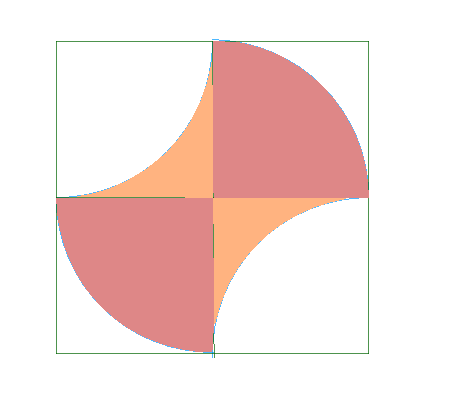
\includegraphics[width=6.5cm]{./svg/pdf/23-24-s3-i-p18-s.pdf}
        \end{center}
    \end{minipage}
\end{figure}

\begin{proof}
    Similar to the Example 8 in the second part of this article series,
    but splitting into four regions, it is easy to see that they all make up two quarter square,
    thus the ratio is $\frac{1}{2}.$ 
\end{proof}

\begin{example*}[Example 18]
    $ABCD$ is a convex quadrilateral. $E$ and $F$ are points on $BC$ and $DA$ such that $BE = 2 EC,$ $DF = 2 FA.$
    Find the ratio of the area of the shaded region to the area of the quadrilateral.
\end{example*}

\begin{figure}[h]
    \centering
    \begin{minipage}[t]{6.5cm}
        \begin{center}
            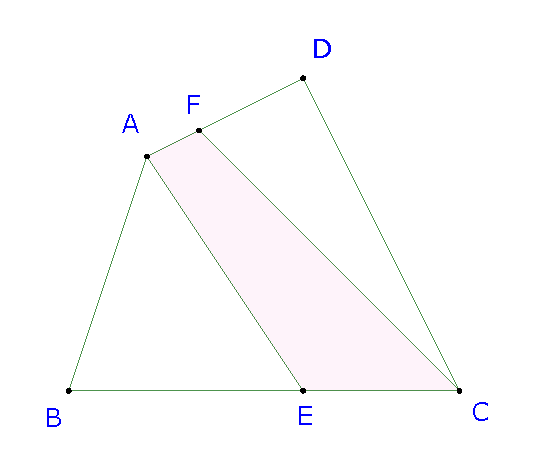
\includegraphics[width=6.5cm]{./svg/pdf/23-24-s3-i-p19.pdf}
        \end{center}
    \end{minipage}
    \qquad
    \begin{minipage}[t]{6.5cm}
        \centering
        \begin{center}
            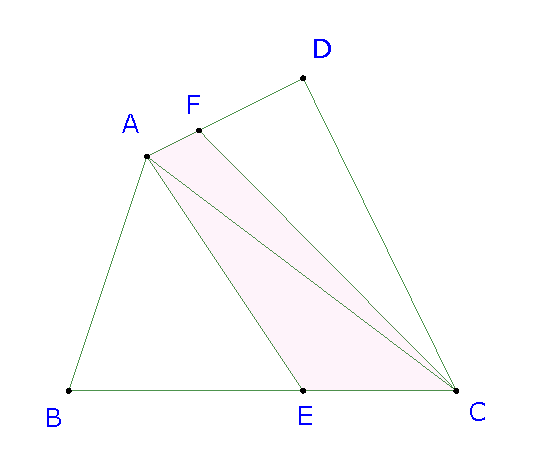
\includegraphics[width=6.5cm]{./svg/pdf/23-24-s3-i-p19-s.pdf}
        \end{center}
    \end{minipage}
\end{figure}

\begin{proof}
    Connect $AC.$ Since $BE = 2EC$ and $DF = 2 AF,$
    \[
        \begin{aligned}
            &\frac{[ACE]}{[ABC]} = \frac{[CFD]}{[CAD]} = \frac{[ACE] + [CFD]}{[ABC] + [CDA]} = \frac{[ACE] + [CFD]}{[ABCD]}\\
            &\Rightarrow \frac{[AECF]}{ABCD} = 1 - \frac{[ACE] + [CFD]}{[ABCD]} =  \frac{1}{3}.
        \end{aligned}
    \]  
\end{proof}

\newpage

\begin{example*}[Example 19]
    $ABCD$ is a square. $E$ and $F$ are midpoints of $BC$ and $CD.$
    $BF$ intersect $AE$ and $AC$ at $G$ and $H$.
    Find the ratio of the area of the shaded region to the area of the square.
\end{example*}

\begin{figure}[h]
    \centering
    \begin{minipage}[t]{6.5cm}
        \begin{center}
            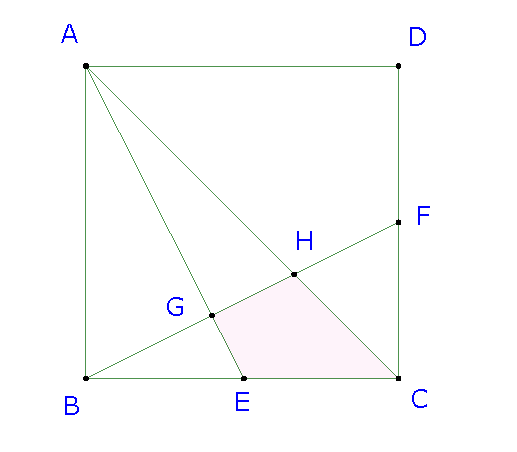
\includegraphics[width=6.5cm]{./svg/pdf/23-24-s3-i-p20.pdf}
        \end{center}
    \end{minipage}
    \qquad
    \begin{minipage}[t]{6.5cm}
        \centering
        \begin{center}
            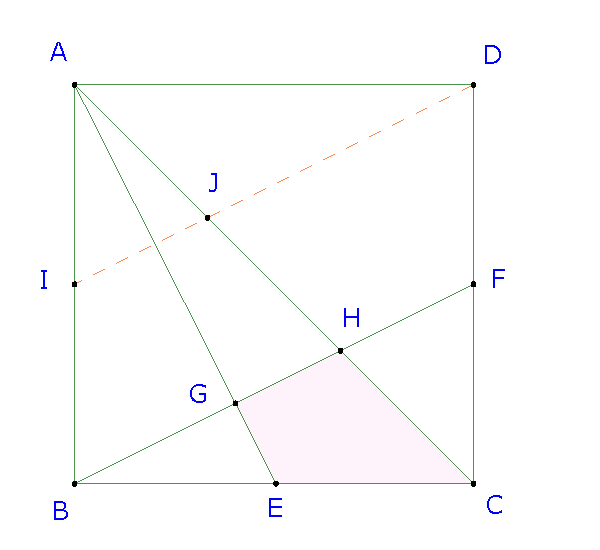
\includegraphics[width=6.5cm]{./svg/pdf/23-24-s3-i-p20-s.pdf}
        \end{center}
    \end{minipage}
\end{figure}

\begin{proof}
    WLOG, let the side length of the square be 1. $BE = \half,$ $AE = \sqrt{AB^2+BE^2} = \frac{\sqrt{5}}{2}.$
    \[
        \begin{aligned}
            &\triangle BGE \sim \triangle ABE \Rightarrow \frac{[BGE]}{[ABE]} = \left( \frac{BE}{AE} \right)^2 
            = \left( \frac{\half}{\frac{\sqrt{5}}{2}} \right)^2 = \frac{1}{5} \Rightarrow [BGE] = \frac{1}{20}.\\
            &[CFH] = \frac{HF}{DJ}[CJD] = \frac{1}{4}[CJD] = \frac{1}{4}\frac{CJ}{AC} [ACD] = \frac{1}{6}[ACD] \Rightarrow [CFH] = \frac{1}{12}\\
            &\Rightarrow [GHCE] = [BCF] - [BGE] - [CFH] = \frac{1}{4} - \frac{1}{20} - \frac{1}{12} = \frac{7}{60}
        \end{aligned}
    \]
    Thus, the ratio is $\frac{7}{60}.$
\end{proof}

\newpage

\begin{example*}[Example 20]
    (\textit{10 points}) In the diagram below two perpendicular diameters divide a circle into four parts.
    On each of these diameters a circle of half the diameter is drawn, tangent to the original circle and meeting at its centre.
    A radius to the large circle is drawn through the intersection points of these smaller circles.
    Show that the red and blue shaded regions are of the same area.
\end{example*}

\begin{figure}[h]
    \centering
    \begin{minipage}[t]{7.5cm}
        \begin{center}
            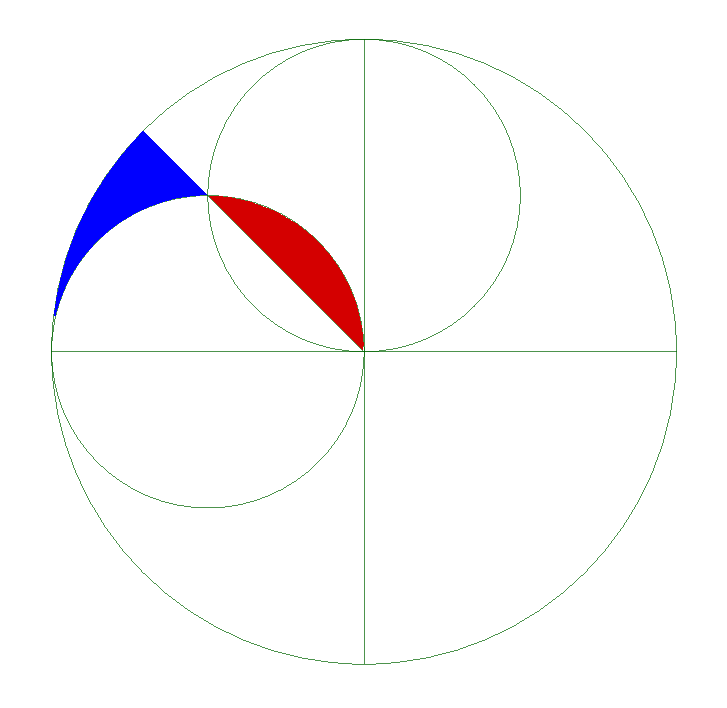
\includegraphics[width=7.5cm]{./svg/pdf/23-24-et-a-p3.pdf}
        \end{center}  
    \end{minipage}
    \qquad
    \begin{minipage}[t]{7.5cm}
        \centering
        \begin{center}
            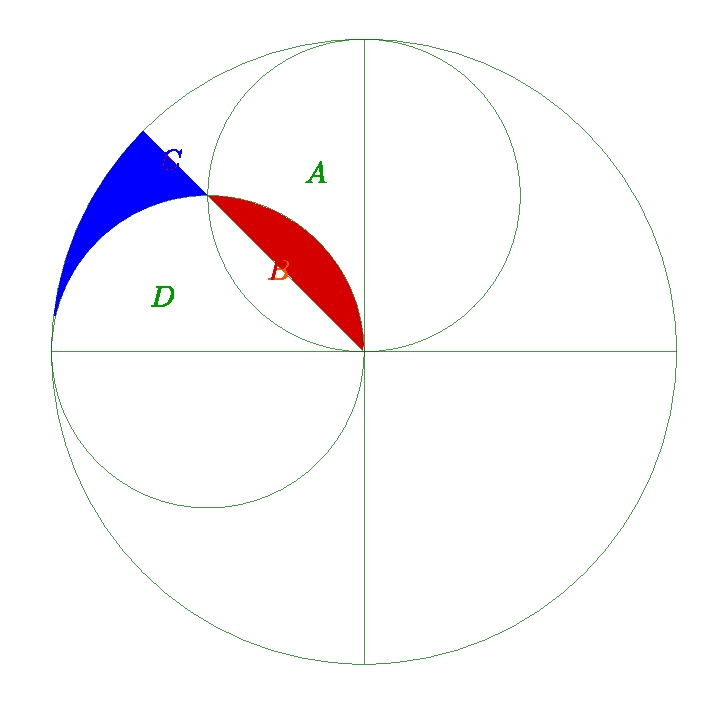
\includegraphics[width=7.5cm]{./svg/pdf/23-24-et-a-p3-s.pdf}
        \end{center}  
    \end{minipage}
\end{figure}


\begin{soln}
    Let $A, B, C,$ and $D$ denote the regions in the figure above. Let $[X]$ denotes the area of a region $X.$
    \[
        [A] + [C] = \frac{1}{4} \pi (2r)^2 - ([B] + [D]) = \frac{1}{4} \pi (2r)^2 - \frac{1}{2} \pi r^2 = \frac{1}{2} \pi r^2 = [A] + [B]
    \]
    Thus $[B] = [C],$ or $\boxed{\half[B]=\half[C].}$
\end{soln}


\end{document}